%%%%%%%%%%%%%%%%%%%%%%%%%%%%%%%%%%%%%%%%%%%%%%%%%%%%%%%%%%%%%%%%%%%%%%%%%%%%%%%%
%2345678901234567890123456789012345678901234567890123456789012345678901234567890
%        1         2         3         4         5         6         7         8

\documentclass[letterpaper, 10 pt, conference]{ieeeconf}  % Comment this line out
                                                          % if you need a4paper
%\documentclass[a4paper, 10pt, conference]{ieeeconf}      % Use this line for a4
                                                          % paper

\IEEEoverridecommandlockouts                              % This command is only
                                                          % needed if you want to
                                                          % use the \thanks command
\overrideIEEEmargins
\usepackage{xcolor}
\usepackage{amsmath}
\usepackage{graphicx}
\newtheorem{theorem}{Theorem}
\newtheorem{statement}{Statement}
\newtheorem{lemma}{Lemma}

\newenvironment{solution}[1][\it{Solution}]{\textbf{#1.} }{$\square$}
\DeclareMathOperator*{\argmin}{arg\,min}
% See the \addtolength command later in the file to balance the column lengths
% on the last page of the document



% The following packages can be found on http:\\www.ctan.org
%\usepackage{graphics} % for pdf, bitmapped graphics files
%\usepackage{epsfig} % for postscript graphics files
%\usepackage{mathptmx} % assumes new font selection scheme installed
%\usepackage{times} % assumes new font selection scheme installed
%\usepackage{amsmath} % assumes amsmath package installed
%\usepackage{amssymb}  % assumes amsmath package installed

\title{\LARGE \bf
Reputation and Spectrum Data Fusion Mechanism...
}

%\author{ \parbox{3 in}{\centering Huibert Kwakernaak*
%         \thanks{*Use the $\backslash$thanks command to put information here}\\
%         Faculty of Electrical Engineering, Mathematics and Computer Science\\
%         University of Twente\\
%         7500 AE Enschede, The Netherlands\\
%         {\tt\small h.kwakernaak@autsubmit.com}}
%         \hspace*{ 0.5 in}
%         \parbox{3 in}{ \centering Pradeep Misra**
%         \thanks{**The footnote marks may be inserted manually}\\
%        Department of Electrical Engineering \\
%         Wright State University\\
%         Dayton, OH 45435, USA\\
%         {\tt\small pmisra@cs.wright.edu}}
%}

\author{Alessandro Galeazzi$^{1}$ Leonardo Badia$^{1}$ and Shu-Chung Chang$^{2}$% <-this % stops a space
\thanks{*This work was not supported by any organization}% <-this % stops a space
\thanks{$^{1}$Department of Information Engineering, University of Padova}%
\thanks{$^{2}$ Graduate Institute of Communication Engineering, Department of Electrical Engineering, National Taiwan University}%
}


\begin{document}



\maketitle
\thispagestyle{empty}
\pagestyle{empty}


%%%%%%%%%%%%%%%%%%%%%%%%%%%%%%%%%%%%%%%%%%%%%%%%%%%%%%%%%%%%%%%%%%%%%%%%%%%%%%%%
\begin{abstract}
Cognitive Radio Network appears to be one of the suitable technologies to realize shared accesses of licensed spectrum by secondary users for increasing spectrum efficiency. One main advantage of Cognitive Radio Network is the possibility to implement a distributed
cooperative spectrum sensing mechanism.
Although it has been proven that the distributed
sensing paradigm has many advantages respect to a centralized approach, it leaves
rooms for new security threats such as Spectrum Sensing Data Falsification attack. In this work we design a new mechanism that exploits sensing correlation through the concept of reputation. By both theoretical analysis and simulations, we show that our mechanism is able to reduce the spectrum decision error rate while it does not introduce any new threats.
\end{abstract}


%%%%%%%%%%%%%%%%%%%%%%%%%%%%%%%%%%%%%%%%%%%%%%%%%%%%%%%%%%%%%%%%%%%%%%%%%%%%%%%%
\section{INTRODUCTION}
In the past 20 years the number of devices connected to the Internet has been increasing and recent forecasts estimate that both internet traffic and device number will keep growing up in the next years. In particular, it is predicted that the fully implementation of IoT paradigm will boost the connectivity demand\cite{cisco}. In order to provide connection to a massive amount of devices, additional spectrum resources are needed\cite{khasawneh}. 
Moreover, many authors pointed out that the current static allocation of spectrum resources leads to a low spectrum efficiency and utilization\cite{kha13},\cite{leon}. Many regulatory bodies introduced the idea of spectrum sharing\cite{peha} to mitigate this problem.
According to this paradigm, part of the spectrum should not be reserved to a licensed user that has the exclusive access to it, but secondary users can opportunistically transmit in the same band, provided that they do not cause any harmful interference to the licensed Primary User (PU)\cite{rome}. In this scenario, it becomes crucial to assess whether PU is transmitting or not. 
Among all the approaches proposed to detect PU transmission, it has been proven that the distributed sensing paradigm can effectively improve the system detection capability and solve some sensing problem found in centralized approaches\cite{leon}. However, a new security threat, called Spectrum Sensing Data Falsification(SSDF) attack, arises\cite{cabric},\cite{khasawneh}. This offensive takes place when one or more corrupted secondary devices, also named Malicious Secondary Users(MSUs), report fake spectrum occupancy information in order to disrupt the cooperative sensing paradigm and induce wrong decision on channel occupancy\cite{leon}. 
%A wrong spectrum decision can, on one hand, cause unacceptable interference to licensed user, on the other reduce the communication opportunity and hence the throughput of the network\cite{rawat}.
There is hence the need for a mechanism able to mitigate the effects of MSUs presence. In this paper we propose and analyze the performance of a new mechanism for securing the distributed sensing of CRN. Exploiting the concept of reputation and the channel correlation among devices, we show that our mechanism is able to enhance the system security if there is enough correlation among SUs. The paper is organized as follow. Section \ref{sec2} is dedicated to the analysis of the research literature, in section \ref{sec3} the scenario assumption, the mechanism and its mathematical formulation are introduced. Section \ref{sec4} shows the results and their analysis, conclusion and future work can be found in \ref{sec5}.
%%%%%%%
\section{Related works}
\label{sec2}
Some countermeasures for Malicious users identification in SSDF attack and selfish behavior prevention have already been proposed. In \cite{qingao} it is show how it is possible to exploit channel spatial correlation in order to identify malicious user through low rank matrix completion algorithm. This mechanism encodes the devices decisions about channels into a matrix and then applies an iterative algorithm in order to identify and disqualify malicious users. A rank estimation algorithm and an estimation strategy for the number of corrupted channels are required to avoid the need of prior information about the channel and environment from third parts. This increase the complexity of the method, that requires a non negligible computational power when the number of devices becomes large.
    
In \cite{taoqin} a beta reputation based trust aware decision mechanism is proposed. Exploiting Beta reputation system, i.e. a reputation estimator based on beta distribution, the authors build a defense mechanism for CRN. This mechanism consider a history of decision and time discount factors in order to discount the less recent sensing, but they also introduce high penalization for device that contribute to wrong decision. In order to assure a reliable feedback, the existence of a Primary User Base Station(PUBS) in addition of a FC is supposed. Moreover, communications between PUBS and FC are possible and indeed necessary in case of a wrong decision that causes interference.

The authors of \cite{rawat} analyze deeply how the presence of Malicious user interferes with the decision taken at the FC. In their work, an analysis on the fraction that makes the FC unable to take meaningful decision is showed and a precise threshold is found. Moreover, they also propose a mechanism for Malicious user identification based on sensing time sequences and decision results.

In \cite{leon} it is underlined how the concepts of trust and reputation are fundamental for implementing a security mechanism against SSDF attack. By exploiting correlations on sensed data, it is possible to increase or decrease the reputation of a SU and eventually ban SUs that obtain a reputation low enough to be considered malicious. Although this can be done by reducing the resources assigned to low reputation SUs, as the authors notice, it is not enough to protect from all malicious user but can effectively incentivize honest SUs to cooperate.
\section{Mechanism Description and Formulation}
\label{sec3}
\subsection{Scenario Assumption}
%%%%%%%%%%%%%%%%%%%%%%%%%%%%%%%%%%%%
%    inserisci img crn scen     %%%%

\begin{figure*}
\centering
\includegraphics[scale=0.5]{figures/CRNscenario.jpg}
\caption{Cosidered Scenario}\label{CRNscen}
\end{figure*}
%                               %%%%
%%%%%%%%%%%%%%%%%%%%%%%%%%%%%%%%%%%%
In this research we do consider the CRN system depicted in \ref{CRNscen} and described in IEEE 802.22 and in the research literature \cite{hyder},\cite{rawat},\cite{najimi},\cite{ghaznavi},\cite{ma},\cite{qingao},\cite{qin}. There are 3 entities: one primary or incumbent user, a fusion center and a set of secondary users that have the capabilities of Cognitive Radio device.

More precisely, we assume the presence of one Primary User(PU) that owns the license to access the spectrum band $B$. We consider $N$ channels in the band $B$ and a PU that can transmit through any of them at any time. The PU shares band $B$ with other users but has a priority over other CR users in accessing spectrum band $B$. We now make some assumption about PUs:
\begin{itemize}
\item {Other entities in the CRN have no specific information and details about PU transmission activities such as PU type, its transmission equipment, its transmission waveform, its location and so on.}
\item{The PU is transmitting from time to time, without any predefined pattern and without signaling its transmission episode to the CRN}
\end{itemize}

Fusion Center (FC) of the CRN is the entity responsible for the spectrum data collection, data fusion according to a fusion rule and the final decision on individual channel occupancy\cite{hyder},\cite{rawat}\cite{ma}. It is also responsible to the CR users allocation in the channels of band B unused by PU. Further, as in \cite{qingao}, we assume the FC capable of splitting all the SUs into subsets based on their positions. A subset of SUs is also called a \textit{location}. FC periodically sends to individual SUs information about which CRs are the neighbors of each SU. For each location, FC request periodically each SUs in the location to provide data about spectrum occupancy and the SU's assessment of neighbors' reputation.
%
Then FC fuses SUs data and makes decision about occupancy according to a fusion rule for each channel over a location. Finally, FC distributes the available resources to SUs. We make the following assumption on FC:
\begin{itemize}
\item {The FC does not have any role in channel sensing. The sensing system does not rely on a central/privileged unit to sense the spectrum.}
\end{itemize}

Secondary Users(SU) are unlicensed CR users that exploit the spectrum holes left by PU to access one or more of the $N$ channels of band $B$. There can be two type of SU: Honest SU(HSU) and Malicious SU (MSU), which can be a subset of HSUs\cite{rawat}\cite{ma}\cite{hyder}. In particular, MSUs are HSUs that are corrupted by an attacher. We make some assumptions on SUs sensing capabilities. Since HSUs and MSUs are the same type of physical devices, both have the same capabilities. We assume that:
\begin{itemize}
\item {A SU can identify the presence of PU and modify their transceiver parameters in order to exploit spectrum holes left by PU.}
\item{For each devices subset, the sensing measurements are strongly correlated. This implies that devices belonging to the same subset have high probability to sense the same spectrum condition\cite{qingao}.}
\item{When a SU is transmitting its spectrum and reputation data to the FC, all device in the same subset are able to listen and correctly decode its transmission.}
\item{each SU can assign a reputation index, i.e. a number between 0 and 1, to all other SUs belonging to the same location, i.e. to all its neighbors.}
\end{itemize}
We now define some notation that will be useful for the next sections. In particular we have:
\begin{equation}
\begin{aligned}
g_{i,j}\equiv & \text{ Probability that SU }j\text{ is honest according to SU }i,\\
&\text{ where SU }i\text{ and }j\text{ are in the same location.}
\end{aligned}
\end{equation}
Different SUs can have different indexes depending on many factor such as what they sensed or if they are MSU or HSU. We also define $g_{i,i}=0$, since in our model it is not relevant the self-judgment of users. Suppose we have $k$ SUs belonging to the same location. For each user $i$, we define the following vector
\begin{equation}
g_i=[g_{i,1},g_{i,2},\dots,g_{i,i-1},0,g_{i,i+1},\dots,g_{i,k}]. 
\label{indexes}
\end{equation}
Thus, $g_i$ is a real vector of length $K$ with each entry in $[0,1]$. 
We now clarify the difference between HSUs and MSUs. We suppose that both HSUs and MSUs use energy detection technique to assess channel occupancy. However, HSUs are ordinary devices that maximizes its own spectrum-time access and reports true information to FC. Thus, we suppose HSUs do not alter spectrum reports, but they can manipulate its reputation indexes in order to obtain more resources. This assumption is justified since a HSU aim to increase its communication opportunities and thus has no incentive for inducing a wrong decision at the FC by altering its spectrum reports. Conversely a MSU aims to induce wrong decision at the FC. It can alter both its spectrum and reputation data in order to reach its scope. Notice that a MSU does not care about the resources FC assigns to it.
\subsection{FC Fusion Rule and System dynamics}
Since each SU assign a reputation index to every SU, due to different assesments a SU can have a wide range to value assigned to it. For example, MSUs can assign 0 to a SUs, while other HSUs give it 1. In order to have a unique reputation value for each SU, there is the need to fuse all the reputation indexes a SU got to obtain one number between 0 and 1. This number should indicate the average reputation of a SUs in the network. 
The mathematical average of all indexes of a SU may not the most appropriate way to calculate it, since, in the mathematical average all the terms have the same weight and, in our scenario, this can lead to a situation in which the index from a SUs that got all 1 weights as much as the one given by a SUs that got all 0. Clearly this is an unwanted behavior for a fusing mechanism.
In order to avoid this, we define define a new quantity, called Global Reputation Index(GRI). GRI gives us a measure of how much reliable is a SU, taking into account all the reputation indexes of the system.
We define the GRI $G_i$ for SU i as: 
\begin{equation}
G_i=\frac{\sum\limits_{l=1}^{k}g_{l,i}\sum\limits_{t=1}^{k}g_{t,l}}{\sum\limits_{h\neq i}\sum\limits_{l=1}^{k}g_{l,h}}
\label{Gindex}
\end{equation}
The formula \ref{Gindex} is the weighted sum of the reputation indexes it got. The weights are the arithmetic average of all reputation indexes a user got. For example, the weight for the term $g_{j,i}$ is $\frac{1}{k-1}\sum\limits_{l=1}^k g_{l,j}$. Notice that the term $\frac{1}{k-1}$ is not in the formula \ref{Gindex}, since it cancels out with the same one at the denominator, where there is the sum of all the weights. Since for definition $g_{i,i}=0$, the column $i$ is excluded from the sum in the denominator, since it is never taken into account in the numerator. In this way FC fuses all the reputation indexes a user got into one unique number. 

Now we describe how the FC uses GRIs to assess channel occupancy and assign resources percentage to SUs. For each SU $i$ in each location, FC receives together with the reputation indexes $g_i$ the channel sensing results. 
We define the results of the sensing of user $i$ on channel $h$ as $C^h_i$. In particular, we have that:
$$
C^h_i=
\begin{cases}
1 \text{ if the channel is sensed busy}\\
0 \text{ if the channel is sensed idle}
\end{cases}
$$
for each user $i\in \{1,2,\dots,K\}$ and for each channel $h \in \{1,2,\dots,N\}$. Hence we can define the binary vector of all sensing results for user $i$ as $C_i=[C^1_i,C^2_i,\dots,C^N_i]$.
%%
With the GRIs and the vectors $C_i$ of each SU $i$ in the location, the FC can infer about channels occupancy. It computes the weighted average of spectrum information, using the GRIs as weights. In this way, spectrum reports provided by SUs that have higher probability of being malicious(i.e. a lower GRI) respect to the others have less possibility to considerably influence the final decision. We hence define the function:
\begin{equation}
\Phi(h)=\frac{\sum\limits_{l=1}^{k}C_{h,l}G_l}{\sum\limits_{l=1}^k G_l}, h=1,2,\dots,N
\label{copp}
\end{equation}
For each channel $h$, FC computes $\Phi(h)$ and compares the results with a predetermined threshold $\tau$. If $\Phi(h)\leq\tau$ the channel is marked as free, otherwise it is labeled as busy.
%%
Moreover, the FC calculates the percentage of resources that is assigned to each SU. We decided to link the resources that a user get to its GRI for two reasons. The first is that, although HSUs cooperate during sensing, we aim to discourage selfish behavior by HSU. The second one is that malicious MSUs should get low reputation indexes from HSUs and thus a lower amount of resources is assigned to them. We hence consider the following formula for calculating the percentage of resources $R_i$ assigned to user $i$:
\begin{equation}
R_i=\frac{G_i}{\sum\limits_l G_l}
\label{res}
\end{equation}
We now describe the dynamics of the system. The sensing cycle is divided in 5 different stages:
\begin{enumerate}
\item{FC Request: FC broadcasts a request for spectrum information to the location of interest.}
\item{Spectrum Sensing: For each of the N channels and by using energy detection technique, the SUs in the location sense the spectrum and decide whether the PU is transmitting.}
\item{Reporting and Listening: sequentially, each SU reports spectrum occupancy and reputation indexes about neighbors to the FC. In this stage, when it is not transmitting, a SU listens to its neighbors that broadcast their data.}
\item{Reputation Updating: After all SU transmitted its data, each SU updates its indexes by comparing the SU's information about spectrum and data broadcast by SUs.}
\item{Final Decision: FC takes final decision about channel occupancy and calculates the percentage of resources assigned to every SU. SUs receives from the FC the list of channels and time that it can use for transmitting its data.}
\end{enumerate}
While steps 1,2 and 5 do not depend on the SUs type, during steps 2 and 3 the actions performed by each SUs strongly depend on their type. For example, HSUs and MSUs may report different channel status even if they sensed the same channel condition. In particular a general framework for the updating rule is described by the following formula:
\begin{equation}
g^{t+1}_{i,j}=\max\{\min\{ g^t_{i,j}+\alpha-\beta \chi_i(C^t_i,C_j^t)-\gamma\psi_i(g^t_i,g^t_j),1\},0\}
\label{upequat}
\end{equation}
In \ref{upequat} three quantities are taken into account during the updating process of the index for user $j$ from user $i$. The first one is the past reputation indexes, $g_{i,j}$, the second one is the function $\chi_i$, which depends on the distance between the two spectrum data vector $C_i$ and $C_j$, the third one is a function $\psi_i$ that depends on the two vectors of reputation indexes $g_i,g_j$. Notice that the functions $\xi_i$ and $\psi_i$ depend on $i$, so that diverse users can have different strategies.

In particular, for MSUs we fix the following updating strategy:
\begin{equation}
g^t_{i,j}=
\begin{cases}
0\text{ if SU j is not malicious}\\
1\text{ otherwise}
\end{cases},
C^t_i=\neg C^t_{is} \forall t
\label{msustrat}
\end{equation}
where $\neg C^t_{is}$ is the opposite of what it sensed, as considered in \cite{leon}. Notice that we assume that MSUs know who is a HSU and who is a MSU, that is, the attack is coordinated.

Given this falsification strategy, in the next section we first analyze the requirements that a HSU's strategy must have in order to discourage selfish behavior among HSUs, and then we propose a strategy that makes the system resilient to the presence of noise and MSUs. Indeed, in a real scenario, the sensing results of each SUs may be different, as results of sensing errors. To model noise, we consider two probabilities, $P_d$ and $P_f$, that are the probability of detecting the PU when it is transmitting and the probability of false alarm, i.e. the probability of a detection when PU is not transmitting\cite{digham}. We consider that errors during sensing are I.I.D. among devices and we assume that the PU may be transmitting w.p $P_{tx}=0.5$. These two last statements are justified by the fact that devices are divided into location based on their physical positions and hence experience the same error probabilities\cite{digham} and that we have no information about PU activity.
%%%%%%%%%%%%%%%%%%%%%%%%%%%%%%%%%%
%%%%%%%%%%%%%%%%%%%%%%%%%%%%%%%%%%
\section{Results}
\label{sec4}
\subsection{Perfect Sensing Nash Equilibrium}
The first question we address is how the HSUs should behave in order to guarantee that no one has incentive to adopt a selfish behavior. We start with the perfect sensing case and the presence of only HSU. We use a game theoretic approach to demonstrate that a HSU has no unilateral incentive to alter its reputation indexes in order to obtain more resources, which implies that HSUs reports contains fair sensing and reputation data.
%%%%%
We start considering the process as a dynamic multistage game\cite{tadel}. At each stage the players, i.e. the SUs, choose their actions, i.e. the reputation and spectrum data, based on the information they got in the previous stage and the sensed spectrum condition. We model HSU payoff as the percentage of resources they got, as described in \ref{res}. We use the concept of Nash equilibrium to demonstrate that, under some assumptions on HSUs, behaving in a selfish way for gaining more resource is not rational\cite{tadel}. Since our game may last for an infinite amount of time, we rely on the overtaking criteria\cite{rub} to compare different strategy.
To sum up, our game is made by
\begin{itemize}
\item {Players: K HSUs}
\item {Payoff Function: equation \ref{res}}
\item {Perfect Information: all users knows how the reputation index are fused, that is, they know equations \ref{Gindex} and \ref{res}, and they know the reputation indexes other SUs assigned to them at the end of each stage}
\item{Infinite game: they know that the game is repeated infinitely many times and they do not discount the future payoffs}
\item{They have the same beliefs about others behavior. In particular, we assume that if a HSU $i$ in the previous stage of the game gave indexes $\delta_{i,1},\delta_{i,2},\dots,\delta_{i,k}$, then other HSUs react giving it a reputation index of $\min\limits_{j=1,\dots,k}\delta_{i,j}$ in the current stage.}
\end{itemize}
Notice that our last assumption follows from the rationality of HSUs. Indeed, if a SU $i$ gives a index $g_{i,j}=\delta<1$ to user $j$, the GRI of user $j$ decrease. Hence, it will react by giving a reputation of $g_{j,i}=\delta$. Other HSUs  will do the same, since a lower reputation index for user $j$ means a lower weight of its assessments and thus a lower GRI for them. Moreover, assigning user $i$ a lower reputation index gives them a higher GRI, without fall into any risk of punishments by others.
From now on, we refer to $R^t_i$ as one stage reward or payoff for SUs $i$, $R^{2t}_i=R^t_i+R^{t+1}_i$ as the two stage reward for user $i$ and so on. 
We have the following three lemmas.
%%%%%%%%
\begin{lemma}{Two stage deviation}\\
\label{twostage}
If $K>3$, there is no $\delta<1$ s.t. $R^{2t}_i>\frac{2}{k}$ if $g^t_i=g^{t+1}_i=\delta$ and $g^t_{-i}=1,g^{t+1}=\delta$.
\end{lemma}
Using this lemma, one can demonstrate that 
\begin{lemma}{Multi stage deviation}\\
\label{multistage}
There is no sequence of $\delta^t,\delta^{t+1}\dots,\delta^{t+n}\neq1,1,\dots,1$ s.t.
$g^t_i=\delta^{t},g^{t+1}_i=\delta^{t+1},\dots,g^{t+n}_i=\delta^{t+n}=\delta^t$ $R^{nt}_i>\frac{n+1}{k}$.
\end{lemma}
The last lemma we need is the following.
\begin{lemma}{Infinite stage deviation}\\
\label{infinitestage}
For any sequence $g^{t}_i>g^{t+1}_i>g^{t+2}_i\dots$ $\exists T$ s.t. $R^{t+l}_i<\frac{1}{k}$ $\forall l\geq T$ 
\end{lemma}
%%%%%%%
%%%%%%%
%%%%%%%%%%%%%%%%%%%%%%%%%%%%%%%%%%%%%%%
%%%%%%%%%%%%%%%%%%%%%%%%%%%%%%%%%%%%%%%%
With these lemmas, we can now demonstrate the following theorem.
\begin{theorem}
\label{theo1}
Suppose we have:
\begin{itemize}
\item{Perfect channel correlation among neighbors, that is, $P_d=1,P_f=0$}
\item{No MSU in the system}
\item{At least 4 SUs, i.e. $K\geq 4$}
\item{Rational behavior of HSUs, as defined before}
%\item{If a HSU $i$ in the previous stage of the game gave indexes $\delta_{i,1},\delta_{i,2},\dots,\delta_{i,k}$, then other HSUs react giving it a reputation index of $\min\limits_{j=1,\dots,k}\delta_{i,j}$ in the current stage}
\end{itemize}
Then when each HSU gives reputation 1 to each other is a Nash Equilibrium. 
\end{theorem}
%%%%
%%%%
\begin{proof}
Since HSUs plays the game indefinitely many times, they care not only about the resources they get in the present stage, but also the resources that FC will assign to them in next round when they decide their strategy. Thus, in order to prove the theorem, we show that any unilateral deviation from the strategy $g_{i,j}=1$ does not lead to any advantage. To compare rewards for infinite strategy, we adopt the overtaking criterion\cite{rub}, defined as follow.
Consider two infinite strategy, $\delta=\delta_1,\delta_2,\dots$ and $\delta'=\delta'_1,\delta'_2,\dots$. We will say that the strategy $\delta$ is preferred to $\delta'$ if
\begin{equation}
0<\liminf_{T \to \infty}\sum\limits_{t=1}^T(R^t(\delta'_t)-R^t(\delta_t))
\end{equation}
Where $R^t(\delta_t)$ is the reward for time t playing strategy $\delta$. With an abuse of notation, we will write $\delta^t$ instead of $R^t(\delta_t)$ when comparing strategy with overtaking criterion.
Consider the strategy $E=e_1,e_2,e_3,\dots$ where $e_t=1$ $\forall t$. It is straightforward to see that $R^t=\frac{1}{k}$ for every $t$ and every HSU when they play E. Now consider any other strategy $\delta=\delta_1,\delta_2,\dots$ s.t. $\exists t, \delta_t\neq e_t$.  Thus, $\delta$ must have at some point a deviation from the equilibrium strategy E. We have three cases:
\begin{itemize}
\item {$\delta$ is a two stage deviation that stays forever at a value $\delta^*$ less then one: $\delta=\dots,1,1,\delta^*,\delta^*,\dots$ Then we have
\begin{equation}
\liminf_{T \to \infty}\sum\limits_{t=1}^T(e_t-\delta_t)=+\infty
\end{equation} since after the first step, we the difference is always greater than 0, due to what found in lemma \ref{twostage}.} 
\item{$\delta$ deviates from E only for a finite number of steps. Then there must be a set of index $t_1,t_2,\dots,t_h$ s.t. $\delta_{t_1}<1,\delta_{t_2}<1,\dots,\delta_{t_h}<1$ and $\delta_{t_h+1}=1$. We demonstrated in lemma \ref{multistage} that in this case  $R^{(h+1)t}(\delta)-R^{(h)t}(\delta)$ is less than $\frac{h+1}{k}$, thus
\begin{equation}
\liminf_{T \to \infty}\sum\limits_{t=1}^T(e_t-\delta_t)>0
\end{equation}
}
\item{$\delta$ has an infinite deviation of the type $1>\delta_{t_1}>\delta_{t_2}\dots$. We demonstrate that there is no sequence of $\delta_t$ that can lead to a reward greater that $\frac{1}{k}$ for an arbitrarily long time, so we have:
\begin{equation}
\liminf_{T \to \infty}\sum\limits_{t=1}^T(e_t-\delta_t)+\infty
\end{equation}
If $\neq L$ s.t. $\delta_t\neq 1$ $\forall t>L$.
}
\end{itemize}
Notice that for lemmas \ref{twostage},\ref{multistage} and \ref{infinitestage}, any other type of strategy is dominated by one of the three described before.
Thus we demonstrated that no unilateral deviation, finite or infinite, leads to advantage for HSU when the overtaking criteria is used and thus this is a Nash equilibrium\cite{tadel}.
\end{proof} 
%%%%%%%%%%%%%%%%%%%%%%%%%%%%%%%%%%%%%%%%

\subsection{MSU impact and HSU noise resilient strategy strategy}
After identifying a strategy for HSUs that leads to a desirable equilibrium in case of no MSUs and perfect sensing condition, we now analyze how the impact of MSUs and noise during sensing can affect the system. The first question to address is how to choose the threshold $\tau$ for the channel occupancy.  
\subsubsection{Channel occupancy threshold}
Consider the case where $l$ users over $k$ give the wrong information due to both reporting errors or to malicious deviation. If the channel is busy, i.e. the PU is transmitting,according to equation \ref{copp} we have that the FC takes the right decision if and only if:
\begin{equation}
\frac{(k-l)\cdot 1+0\cdot l}{k}\geq{\tau}
\label{th1}
\end{equation}
A similar equation can be formulated for the case of idle channel:
\begin{equation}
\frac{(k-l)\cdot 0 +1\cdot l}{k}<\tau
\label{th2}
\end{equation}
By combining \ref{th1} and \ref{th2} and solving the system we have that the optimal threshold is $\tau=0.5$. By selecting this threshold, in case of perfect sensing our system can tolerate up to $\lceil\frac{k}{2}\rceil -1$ MSUs in the system. Notice that this is the maximum amount of malicious users that any distributed system that does not rely on central/privileged unit can tolerate.
%%%%%%%%%%%%%%5
\subsubsection{Probability distribution of the hamming distance between two reports}
We now introduce the possibility of errors in the channel sensing process.
Given the detection probability $P_d$, the false alarm probability $P_f$ and the primary user transmission probability $P_tx$ the sensing error probability on one channel can be expressed as:
\begin{equation}
P_e=(1-P_d)*P_{tx}+(1-P_{tx})*P_f.
\end{equation}
That is, $P_e$ is the probability that a device misdetect the state of one of the $N$ channels. Consider now two devices $i$ and $j$ and their spectrum report on one channel $S_i,S_j$. The probability that there is a mismatch on one channel sensing is given by:
\begin{equation}
P_m=P(S_i=1,S_j=0)+P(S_i=0,S_j=1)
\end{equation}
That can be rewritten as:
\begin{equation}
P_m=2(1-P_{tx})*(1-P_f)*P_f +2P_{tx}*(1-P_d)*P_d
\end{equation}
Now consider the case of N channel and suppose that the probability of mismatch among the two reports is independent and identically distributed for each channel. We have that each channel error can be modeled as r.v. Bernoulli distributed, with probability of success $P_m$. Thus we have that the r.v. $mis_{i,j}=||S_i-S_j||$ is distributed as a Binomial r.v of parameters $P_m$ and $N$.
%%%%%%%%
\subsubsection{Noise resilient HSU strategy}
%%%%%%%%%%%%%%
\begin{figure}
\centering
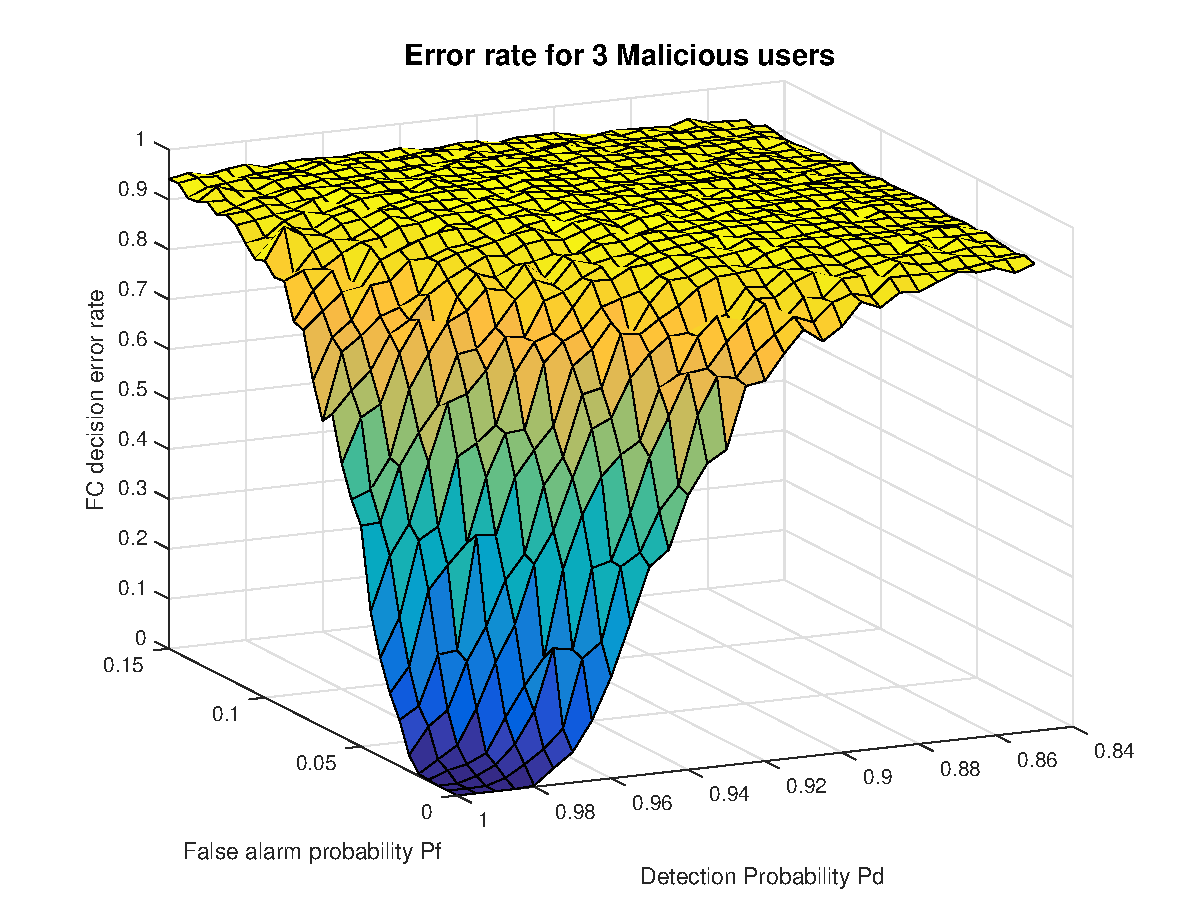
\includegraphics[scale=0.4]{figures/notolerance.eps}
\caption{FC error rate when HSUs uses a strategy that does not consider noise}\label{notolerance}
\end{figure}
%%%%%%%
Although HSUs do not intentionally lie on spectrum reports, there can be difference among their reports due to sensing errors. If a naive strategy that do not take into account sensing errors is used by HSU, the reputation among users easily decrease and reach 0. This happens because as soon there is an error in sensing, the reputation is lowered down. 
In this scenario, MSUs can easily strongly influence the FC decision, as shown in figure \ref{notolerance}%%%%%%%%.
Thus there is the need to design a strategy resilient to sensing errors. We design a strategy that allow SUs to tolerate sensing mistakes up to a certain amount if their behavior follows the rationality condition of \ref{theo1}. 
In particular, we have
\begin{equation}
\label{hsustrat}
g^t_{i,j}=
\begin{cases}
\min\{0.1+g^{t-1}_{i,j},1\}
\text{ if } g_j^{t-1}=g^{*{t-1}}_j,|C_i-C_j|<\xi \\
\max\{ g^{t-1}_{i,j}-\max\limits_h {(g_{i,h}-g_{j,h})}-\frac{|C_i-C_j|}{N},0\}\text{ if not}
\end{cases}
\end{equation}
Where here $g^*$ is the reputation indexes user $j$ should gave according to the common updating rule. Essentially, if a user is updating its reputation according to this updating rule and is not making too much mistakes, its reputation is not lowered down. The increment parameter $\alpha$ is set to 0.1. This is a trade off between the need of a fast recovery of the reputation among devices and the protection against MSUs behavior. The choiche of $\xi$ is based on a statistical analysis of the error distribution. From one hand, one is tempted to set $\xi=N+1$, so that the reputation among HSUs is always maintained. However, this would lead to a simple majority rule wich performance will be taken as a benchmark. On the other hand, a too low threshold for $\xi$ can decrease the reputation among HSUs and thus increase the error rate. Thus, in order to select the most appropriate value for $\xi$, we analyze the distribution of the rv $mis_{i,j}$. On one hand, for HSUs, one want to choose a value for $\xi$ s.t. Pr$(mis_{i,j}>\xi)\approx 0$. On the other, in order to identify MSUs, one want to maximize the probability that the distance between a HSU and MSU reports is bigger or equal to $\xi$. Since MSUs flip each sensing results, the distance between their report is equal to $N$, the number of channels, minus the numbers of sensing mismatch. Since we want to minimize the probability that a MU is unidentified, we can write the condition as Pr$(mis_{i,j}>N-\xi)\approx 0$. Hence the we will select $\xi$ as the solution of the following problem:
\begin{equation}
\xi=\argmin\limits_{x=1,2,\dots,N} (\text{Pr} (mis_{i,j}>N-x)+\text{Pr}(mis_{i,j}>x))
\end{equation}
%%%%%%%%%%%%%%%%%%%%%%%%%%%%%%
\begin{figure}
\centering
\includegraphics[scale=0.4]{figures/prob.eps}
\caption{Distribution of the sum of the two probabilities}\label{probdist}
\end{figure}
%%%%%%%%%%%%%%%%%%%%%%%%%%%%%%
In figure \ref{probdist} is depicted the value of $\text{Pr} (mis_{i,j}>N-x)+\text{Pr}(mis_{i,j}>x)$ for $x=1,2,\dots,10$ and for various values of $P_m$. It is clear how $\xi=5$ is the minimum of the function for all values of $P_m$ and hence it is the best choice when N=10, as set during our simulation.     
%%%%%%%%%%
\subsubsection{Simulation Results}
%%%%%%%%%%%%%%%%%%%%%%%
%#############################

\begin{figure*}[t]
    \centering
    \begin{minipage}[t]{0.32 \textwidth}
     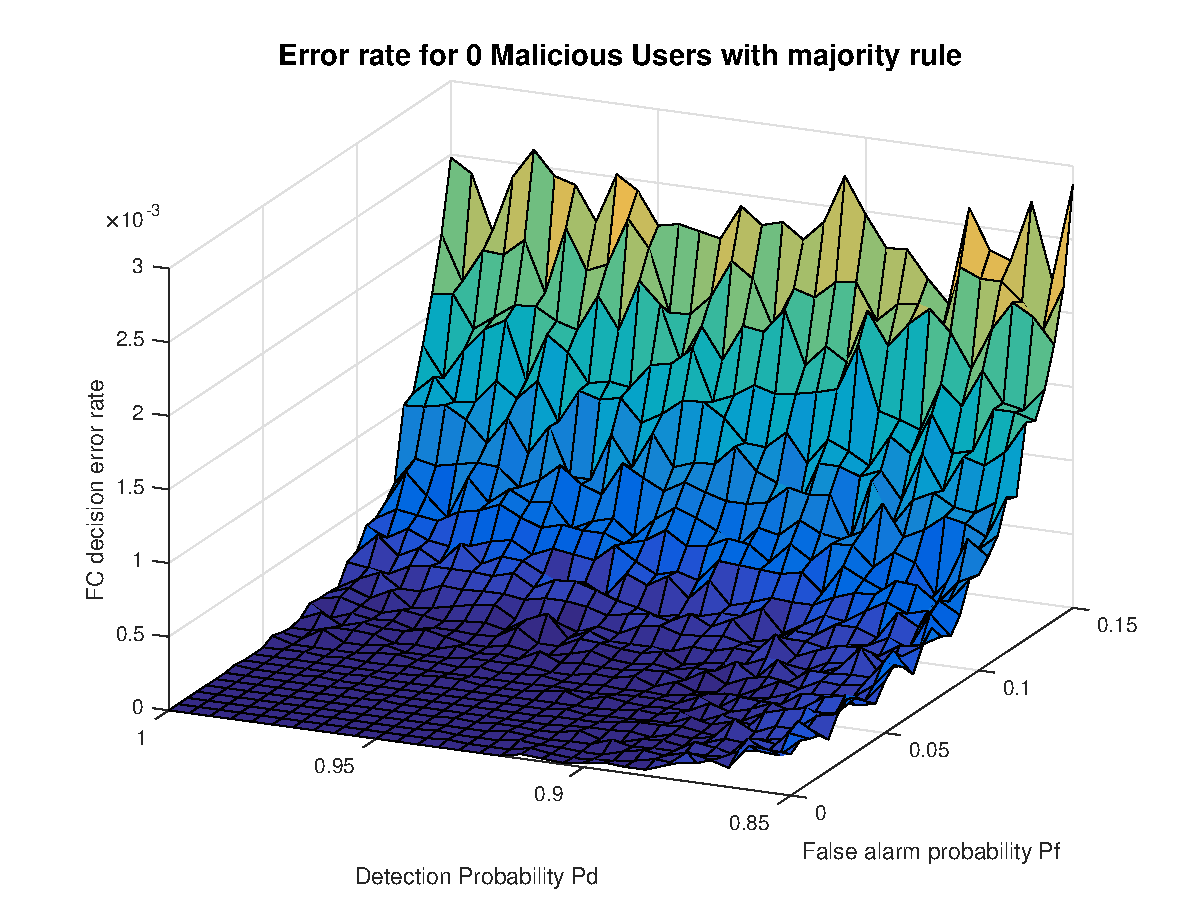
\includegraphics[width=\linewidth]{figures/mr0mu.eps}
\caption{FC decision error rate with majority rule implemented and 0 MSUs }\label{mr0}
    \end{minipage}%
    ~ 
    \begin{minipage}[t]{0.32\textwidth}
        \centering
        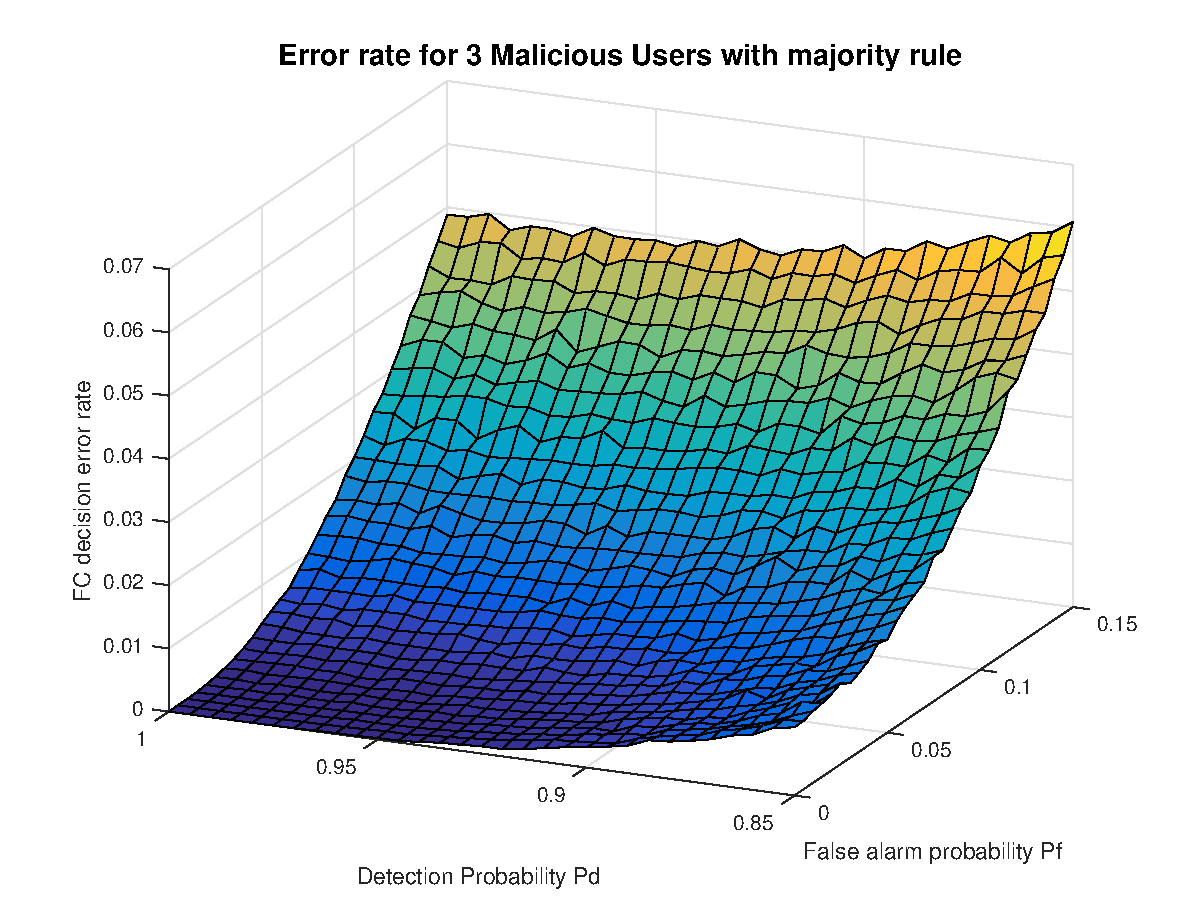
\includegraphics[width=\linewidth]{figures/mr3mu.eps}
        \caption{FC decision error rate with majority rule implemented and 3 MSUs}
        \label{mr3}
    \end{minipage}
    ~
    %
    \begin{minipage}[t]{0.32\textwidth}
        \centering
        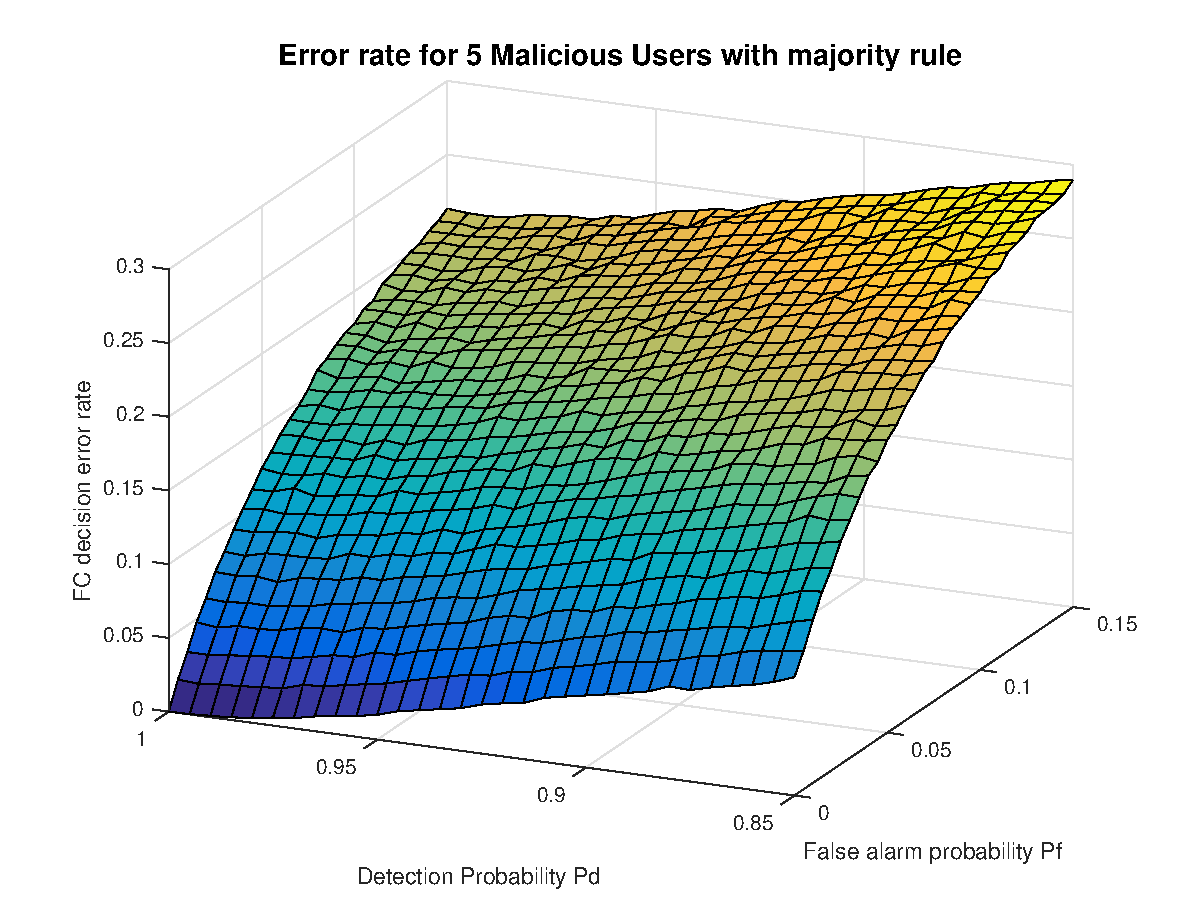
\includegraphics[width=\linewidth]{figures/mr5mu.eps}
        \caption{FC decision error rate with majority rule implemented and 5 MSUs}
        \label{mr5}
    \end{minipage}
    \end{figure*}
    %%%%%%%%
    \begin{figure*}[t]
%#############################%%%
%#############################%%%
%\begin{figure*}[t!]
    \centering
    \begin{minipage}[t]{0.32 \textwidth}
     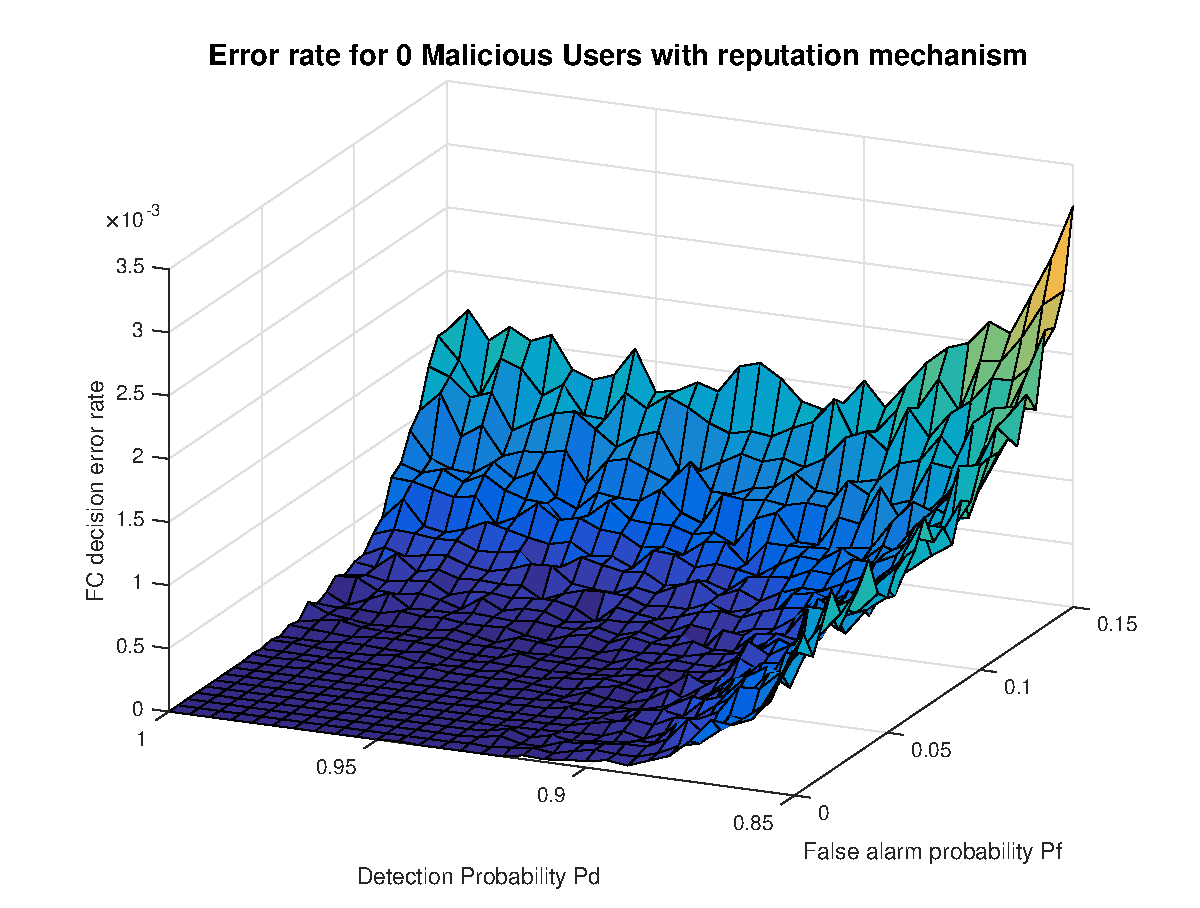
\includegraphics[width=\linewidth]{figures/rm0mu.eps}
\caption{FC decision error rate with reputation mechanism implemented and 0 MSUs}\label{rm0}
    \end{minipage}%
    ~ 
    \begin{minipage}[t]{0.32\textwidth}
        \centering
        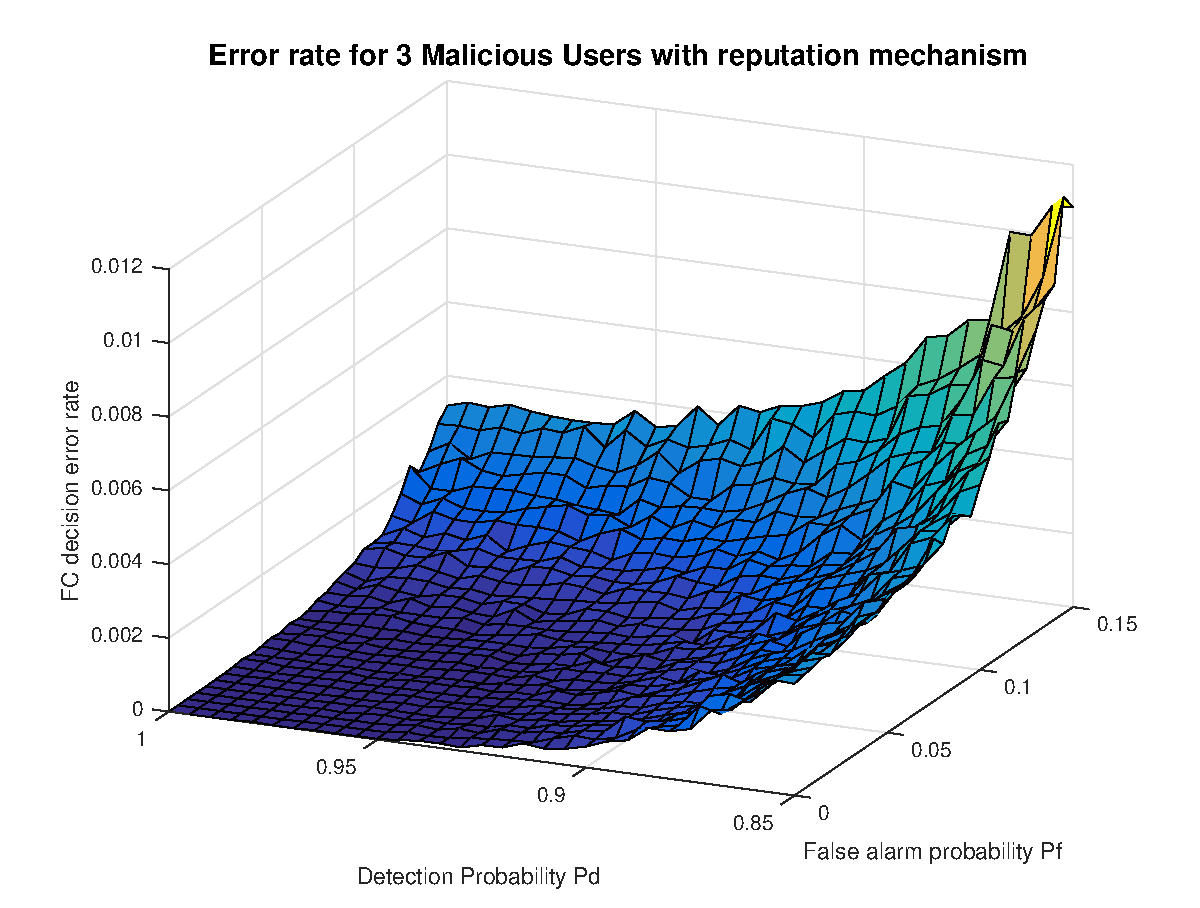
\includegraphics[width=\linewidth]{figures/rm3mu.eps}
        \caption{FC decision error rate with reputation mechanism implemented and 3 MSUs}
        \label{rm3}
    \end{minipage}
    %%%%%%%%
    \begin{minipage}[t]{0.32\textwidth}
        \centering
        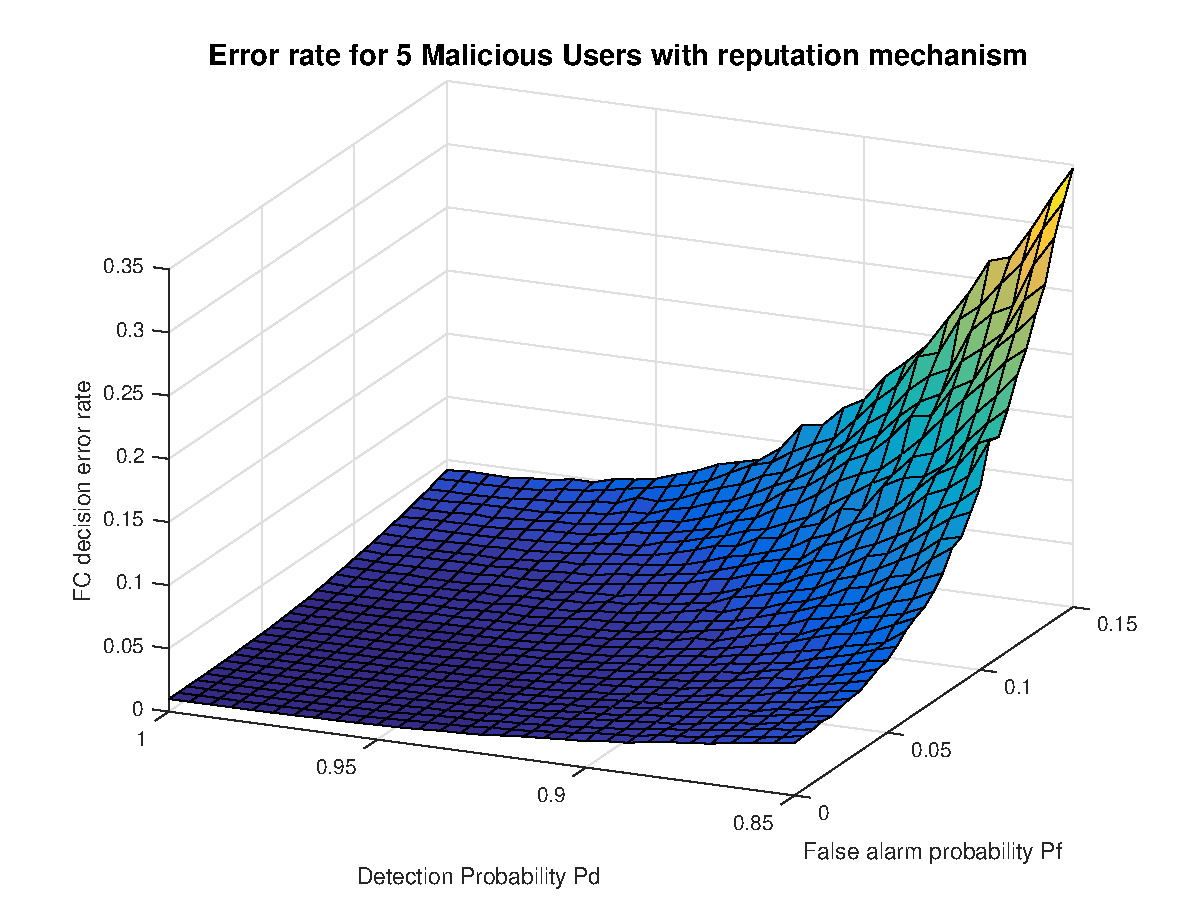
\includegraphics[width=\linewidth]{figures/rm5mu.eps}
        \caption{FC decision error rate with reputation mechanism implemented and 5 MSUs}
        \label{rm5}
    \end{minipage}
    \end{figure*}
    %
    %~ 
    \begin{figure*}[t]

    \begin{minipage}[t]{0.5\textwidth}
        \centering
        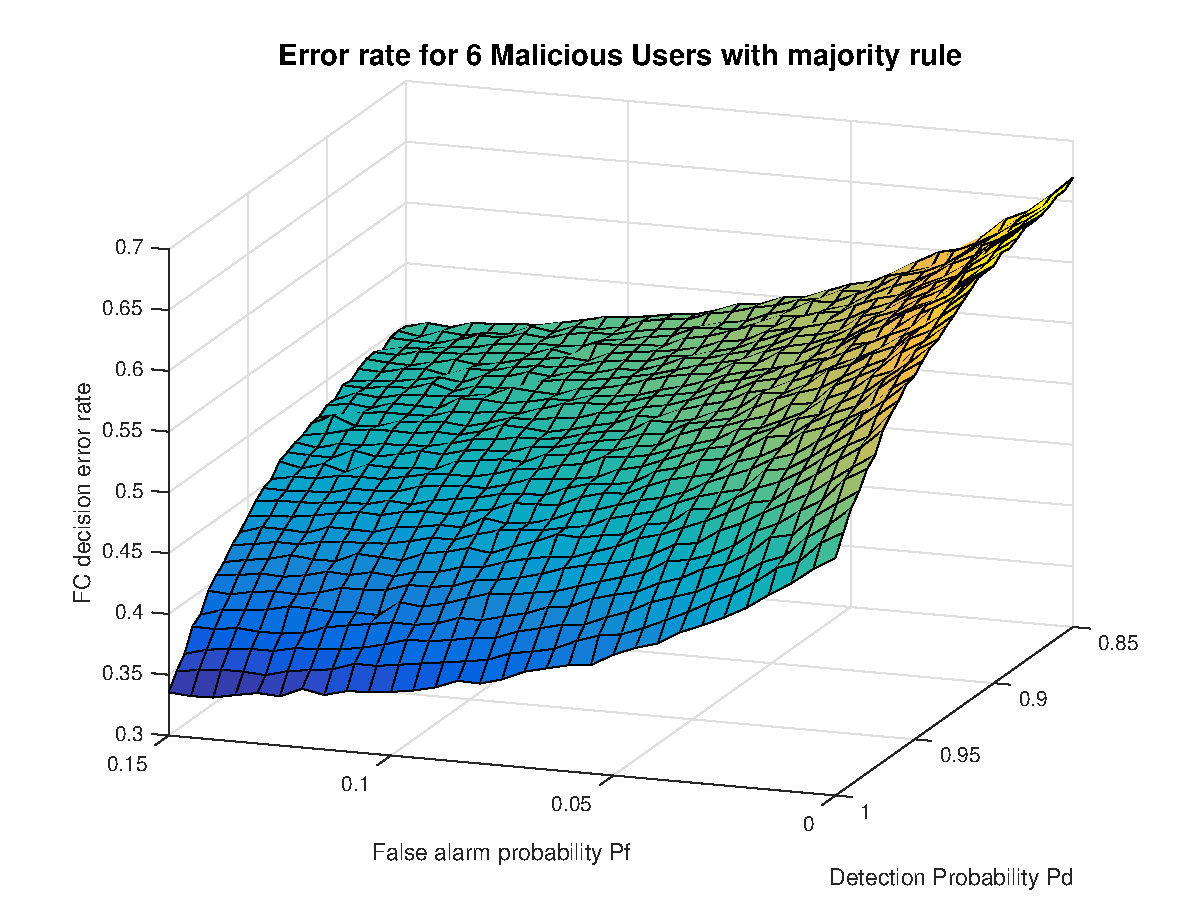
\includegraphics[width=\linewidth]{figures/mr6mu.eps}
        \caption{FC decision error rate with majority rule implemented and 6 MSUs}
        \label{mr6}
    \end{minipage}
    ~ 
    \begin{minipage}[t]{0.5\textwidth}
        \centering
        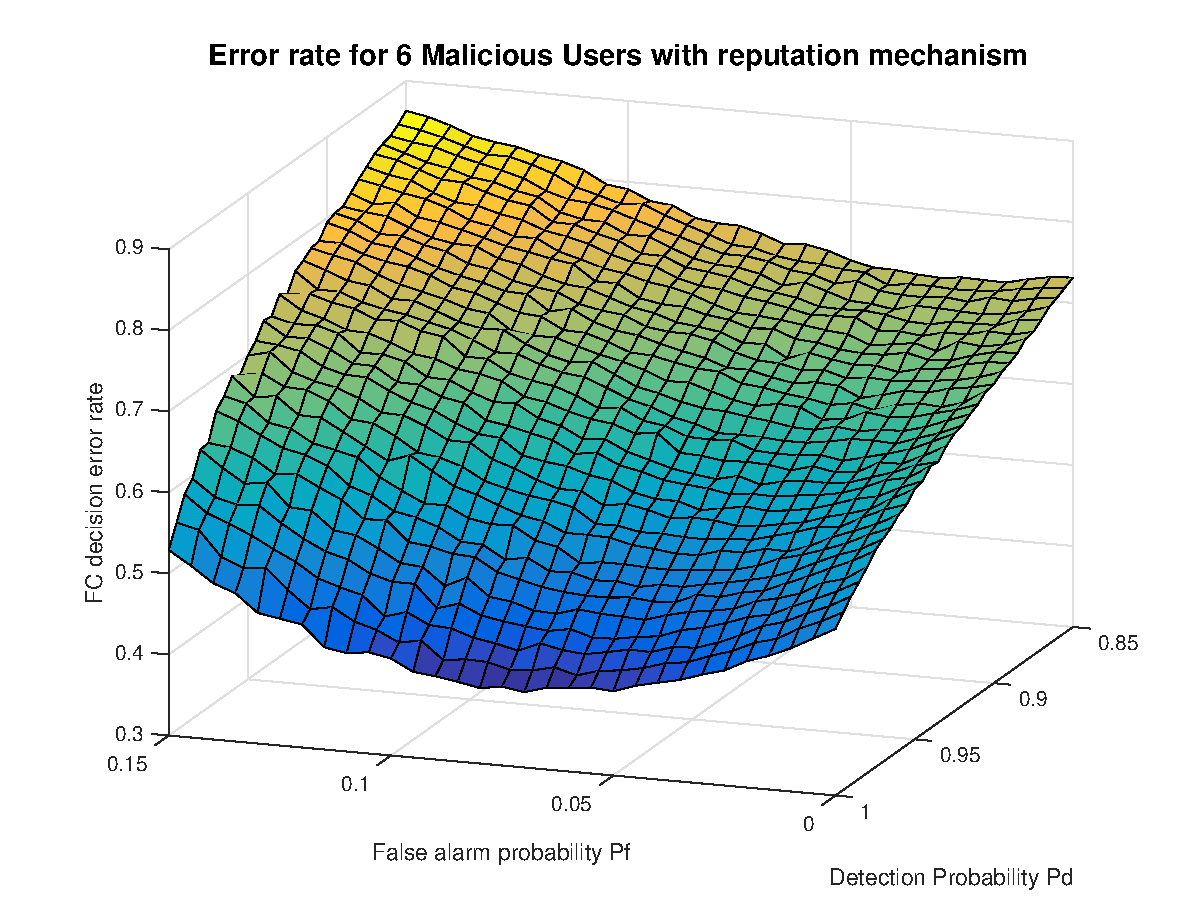
\includegraphics[width=\linewidth]{figures/rm6mu.eps}
        \caption{FC decision error rate with reputation mechanism implemented and 6 MSUs}
        \label{rm6}
    \end{minipage}
\end{figure*}

%############################
%%%%%%%%%%%%%%%%%%%%%%%%%%
In this section we present the results obtained from the simulation of the system. In our scenario, considered $N=10$ channels, $K=12$ users and we let $P_d$ and $P_m$ vary from 1 to 0.85 and from 0 to 0.15 respectively. The transmission probability $P_{tx}$ was set to 0.5 and the threshold $\xi$ to 5. HSUs adopt the updating strategy described in \ref{hsustrat}, while MSUs adopt the strategy described in \ref{msustrat}. In this setting, we focus on FC error rate and how it depends on the amount of MSUs in the system. We vary the number of MSUs from 0 to 6, that is the minimum amount of MSUs that leads to wrong decision at FC at least half of the time. For each setting we run 100 Monte Carlo trials each of 100 sensing round. As a benchmark, we also run the same amount of simulations with a majority rule implemented at FC. The results can be found in figures \ref{mr0},\ref{mr3},\ref{mr5},\ref{mr6},\ref{rm0},\ref{rm3},\ref{rm5} and\ref{rm6}. It can be seen how our mechanism reduces the error rate and mitigate the presence of MSUs respect to our benchmark, but the difference in performance depends on the number of MSUs and the noise level. Indeed, the larger is the number of MSUs in the system, the larger is the gap between our mechanism and the majority rule. Moreover, when the number of malicious user is the maximum theoretically tolerable in a perfect sensing scenario (figures \ref{mr5} and \ref{rm5}) our mechanism has an error rate up to 18\% lower than the benchmark. Further, the shapes of the two curves are substantially different. While the one obtained by a majority rule fusion mechanism increases constantly with $P_m$, our mechanism exhibit a different behavior. Its error rate is low and increases slowly when the values of $P_m$ are low, but rises up very fast after $P_m$ exceed a certain amount. This differences are particularly noticeable when the number of MSUs is high (figures \ref{mr5} and \ref{rm5}). Figures \ref{mr6} and \ref{rm6} show that both systems are not able to efficiently protect the system, even when $P_m$ is low, in presence of 6 MSUs as predicted. In this cases, the asymmetries in the figures are due to the tie breaking rule. In conclusion, our mechanism demonstrated to be efficient in mitigating the MSUs effects, but its performances depends on the level of noise. When the sensing error probability exceed a certain threshold, there is not enought correlation among SUs reports and thus they are not able to penalize MSUs. 
%%%%%%%%%%%%%%%%%%%%%%%%%%%%%%%%%%%%%%%%
\section{Conclusion and Future Work}
\label{sec5}
In this work we propose a mechanism for mitigating the presence of malicious users in a CRN that employs a distributed sensing paradigm to detect PU transmission. Our system exploits the channel correlation among devices thought the concept of reputation to reduce the effects of malicious user presence. By using a game theoretic approach, we demonstrated that the introduction of the reputation reports incentivizes honest users to cooperate at the sensing process without introducing new security threats. We also analyze the effect of noise and malicious users presence on the system and provide details on how to design a noise resilient strategy able to reduce the malicious users damage. Through simulations we show that our mechanism together with the appropriate strategy can reduce the FC error rate respect to a majority fusion rule and is most effective when malicious users and sensing errors are found in the system. However, our simulations also show that the channel sensing correlation assumption cannot be arbitrarily relaxed. This is coherent with our design rationale: we created the mechanism so that spatial correlation can be used to oust malicious users from the network and hence a certain amount of correlation must be present to let the mechanism work properly.
Future works should focus on the optimal strategy for MSU in order to find which equilibrium can be reached and how it depends on malicious users percentage and noise level. 


\addtolength{\textheight}{-12cm}   % This command serves to balance the column lengths
                                  % on the last page of the document manually. It shortens
                                  % the textheight of the last page by a suitable amount.
                                  % This command does not take effect until the next page
                                  % so it should come on the page before the last. Make
                                  % sure that you do not shorten the textheight too much.

%%%%%%%%%%%%%%%%%%%%%%%%%%%%%%%%%%%%%%%%%%%%%%%%%%%%%%%%%%%%%%%%%%%%%%%%%%%%%%%%



%%%%%%%%%%%%%%%%%%%%%%%%%%%%%%%%%%%%%%%%%%%%%%%%%%%%%%%%%%%%%%%%%%%%%%%%%%%%%%%%



%%%%%%%%%%%%%%%%%%%%%%%%%%%%%%%%%%%%%%%%%%%%%%%%%%%%%%%%%%%%%%%%%%%%%%%%%%%%%%%%
%\section*{APPENDIX}

%Appendixes should appear before the acknowledgment.

%\section*{ACKNOWLEDGMENT}



%%%%%%%%%%%%%%%%%%%%%%%%%%%%%%%%%%%%%%%%%%%%%%%%%%%%%%%%%%%%%%%%%%%%%%%%%%%%%%%%
\bibliographystyle{unsrt}
\bibliography{example}
\end{document}
